\begin{itemize}

\item Editor support with keyword highlighting. (Figure \ref{fig:hilight})
	
\item Outline view showing structural members and crosscutting relationships. Also from an advice declaration to the places it advises. (Figure \ref{fig:outline})

\item New \caesarj -project wizard. This wizard helps you to start a new \caesarj -project. (Figure \ref{fig:projectwizard})
  
     
\item \caesarj ~hierarchy view. This view shows the multiple inheritance and nested class relations of an \caesarj ~top level class. (Figure \ref{fig:hierarchy})
  
\item Debugging support. (Figure \ref{fig:debug1})
  
\end{itemize}


\begin{figure*}[htbp]
	\centering
		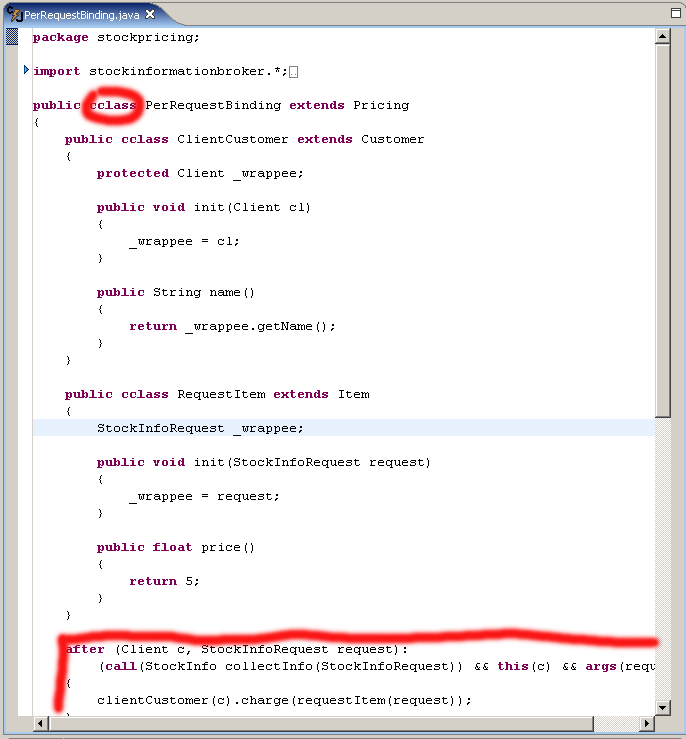
\includegraphics[width=0.60\textwidth]{images/hilight.png}
	\caption{Codehighlighting in \cjdt}
	\label{fig:hilight}
\end{figure*}

\begin{figure*}[htbp]
	\centering
		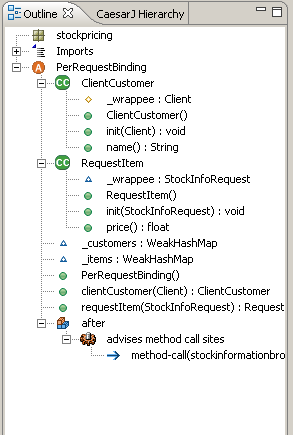
\includegraphics[width=0.35\textwidth]{images/outline.png}
	\caption{Outline view with advice relations}
	\label{fig:outline}
\end{figure*}

\begin{figure*}[htbp]
	\centering
		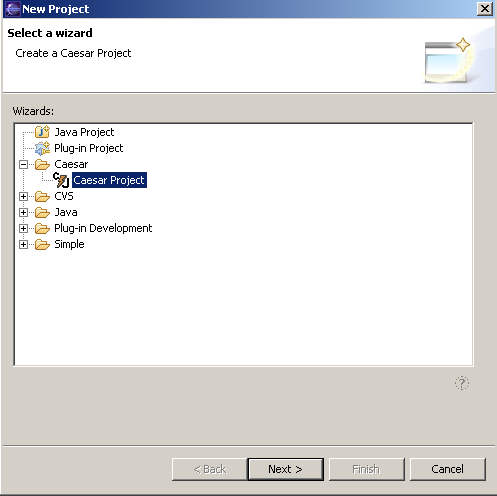
\includegraphics[width=0.60\textwidth]{images/project_wizard.png}
	\caption{New \caesarj -project wizard}
	\label{fig:projectwizard}
\end{figure*} 

\begin{figure*}[htbp]
	\centering
		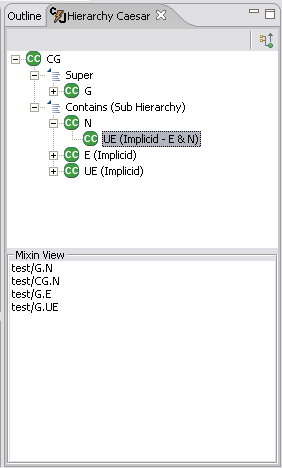
\includegraphics[width=0.35\textwidth]{images/hierarchy.png}
	\caption{\caesarj ~hierarchy view}
	\label{fig:hierarchy}
\end{figure*} 

\begin{figure*}[htbp]
	\centering
		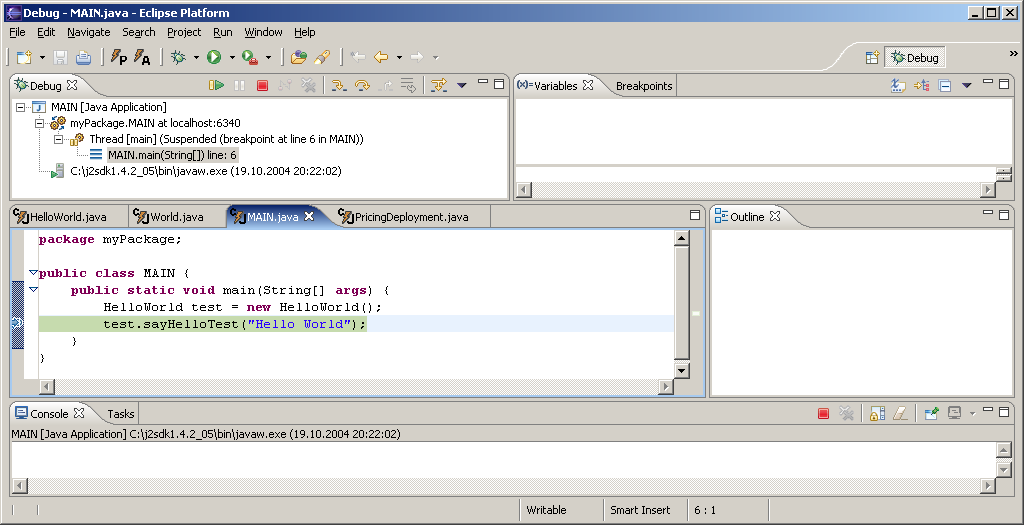
\includegraphics[width=1.0\textwidth]{images/debug1.png}
	\caption{Debugging an \caesarj -project}
	\label{fig:debug1}
\end{figure*}


For detailed description please see Section \ref{features}.